\documentclass[11pt, a4paper,twocolumn]{jarticle}
\usepackage[dvipdfmx]{graphicx}
\usepackage{listings,jlisting}

\begin{document}
%=============================================================
\section{半導体レーザーの発光特性}
\subsection{目的}
この実験の目的は,外部信号により発光パワー変調が可能である半導体レーザーの制御である.
今回は前セメスターのデジタル計測実験でのAD/DAデバイスを用いてパソコンでのプログラムを介してのレーザー制御を行う.
\subsection{手順}
半導体レーザーの赤色導線,黒色導線をそれぞれ電源の5V,GNDに接続し白色導線をAD/DAデバイスに接続した.
キーボード入力により信号電圧(0-5V)を制御するプログラムを記述した.
この時のプログラムはデジタル計測の実験での電圧出力プログラムに定電圧を出力できるように手を加えて流用した.
次に半導体レーザーの前方にパワーメーターを配置し,半導体レーザーの出力を変えながら光パワーを測定した.
また,パワーメータの代わりに前回の実験で作成した受光回路を用いてオシロスコープにて出力電圧を計測した.
さらに,測定した結果をグラフに書き込んだ.
この時受光回路を予め一番強いレーザー光を入射した際に5Vに達して飽和しないように可変抵抗により感度を調節しておいた.

\subsection{結果}
パワーメーター,受光回路で測定した結果は以下のようになった.
ここでパワーメータでは単位はW,受光回路では単位はVのことに注意する.
グラフよりどちらの測定においてもレーザーへの入力電圧が1.2V付近から測定値の増加は緩やかになり飽和していることが読み取れる.
また,パワーメータの飽和点は1.165Vであったのに対し受光回路の飽和点は1.7Vであった.
さらに,パワーメータでの測定ではレーザー出力は0.83Vで初めて検出されたのに対し,受光回路での測定ではレーザー出力は1.05Vで初めて観測された.

\begin{figure}[ht]
 \begin{center}
  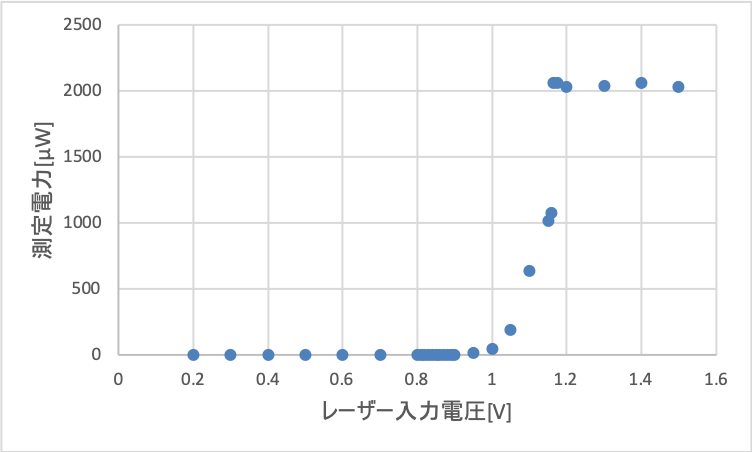
\includegraphics[width=0.8\linewidth]{fig2.png}
 \end{center}
 \caption{パワーメータ測定}
 \label{fig:2}
\end{figure}

\begin{figure}[ht]
 \begin{center}
  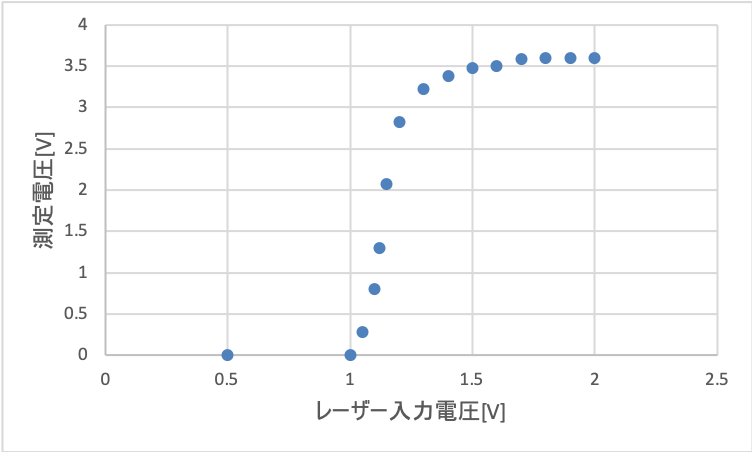
\includegraphics[width=0.8\linewidth]{fig3.png}
 \end{center}
 \caption{受光回路測定}
 \label{fig:3}
\end{figure}

\subsection{考察}
まず二つの測定結果より半導体レーザーが発光するにはある程度の電圧を入力する必要があり,その閾値は1V付近であると考えられる.
またパワーメータと受光回路で初めてレーザー出力が観測される値が異なるのはパワーメータの測定実験後に半導体レーザーのレンズを取り外してしまったため,結果として半導体レーザーの広がり角が大きくなり測定されるまでにより大きな入力電圧を要する必要があったためと考えられる.
さらに受光回路において光パワーを線形的に測定できる範囲はグラフより1.0~1.2Vであると考えられる.

%=============================================================
\newpage
\end{document}
